% From assignment:
% Prioritize measurements and analysis/interpretation!

% Demonstrate use of tools (profiling, ...) , and simple performance
% model.

\section{Measurements}

\subsection{Motivational R-side measurement}

\begin{figure}[!htbp] \centering
  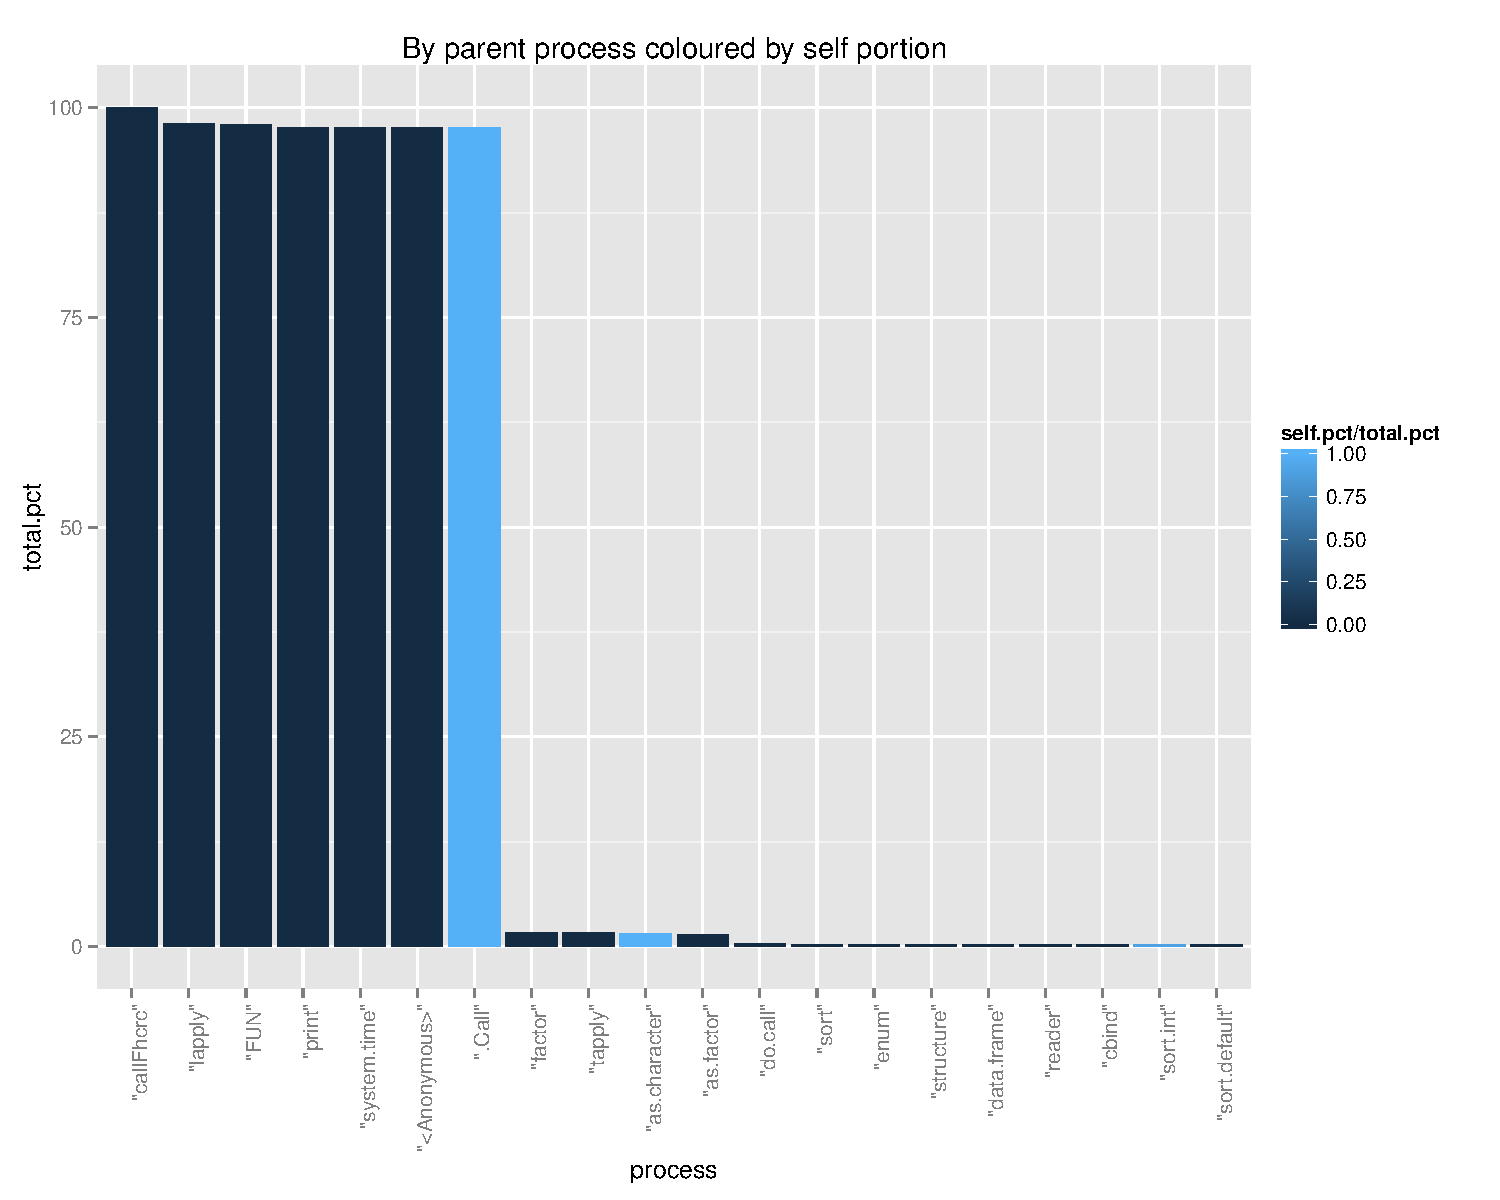
\includegraphics[width=0.7\textwidth]{images/parentColByPortion.pdf}
  \caption{Performance testing on the R side, where the ".Call" is the
C++-code which can be run in parallel.}
  \label{fig:rMot}
\end{figure}
 
To motivate the need and choice to go parallel Figure \ref{fig:rMot}
shows the processes from the R-side where ``.Call'' is the part which
is implemented in C++ and which can be run in parallel. The height of
the bars indicates the time that function takes and the colour
indicates the portion of time spent in the function itself. From
Figure \ref{fig:rMot} we can conclude that ``.Call'' itself
constitutes over 95\% of the time spent.

\subsection{Motivational C++-side measurement}
\begin{figure}[!htbp] \centering
  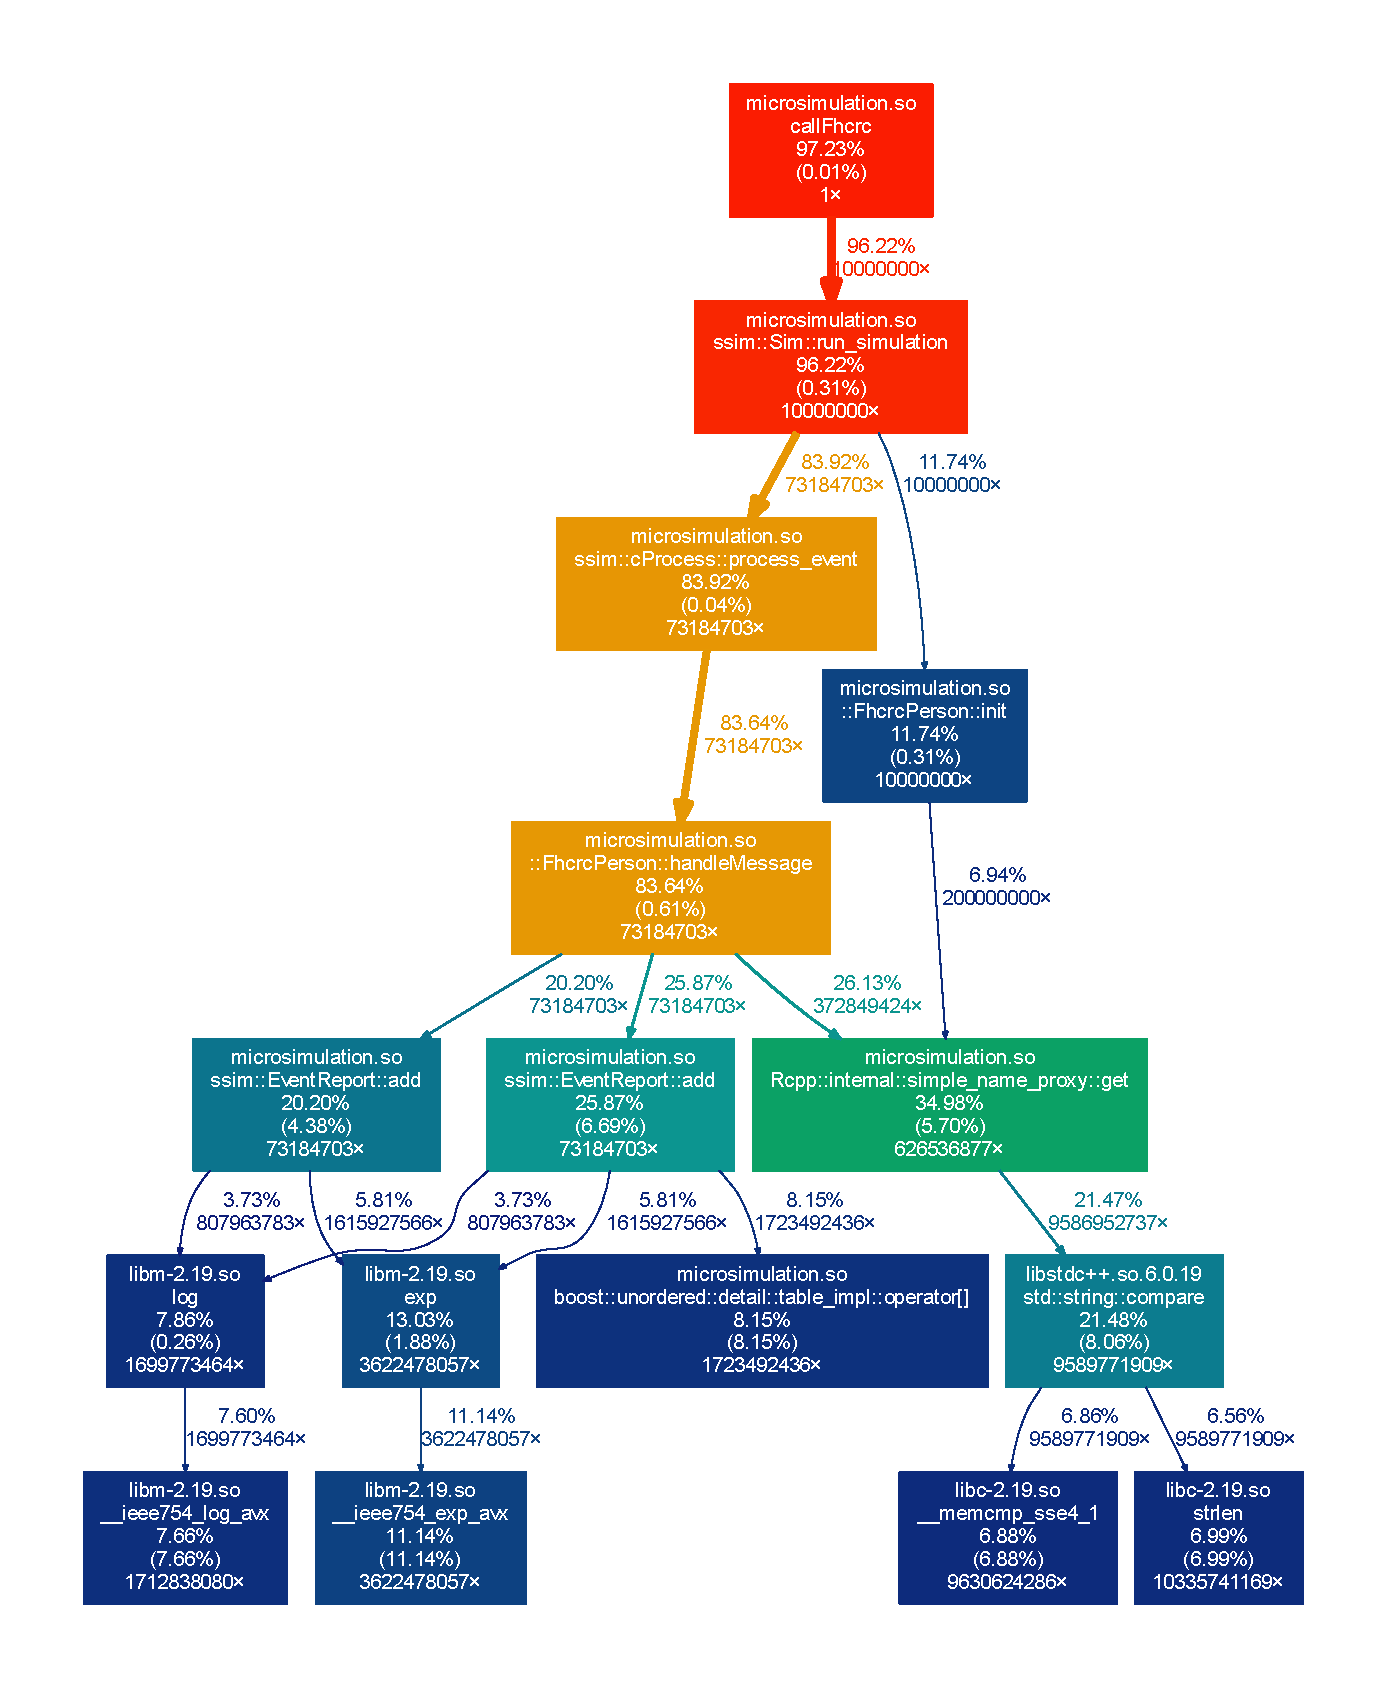
\includegraphics[height=0.70\textheight]{images/simpleMotivatingValgrind.pdf}
  \caption{Using Valgrind to profile the main C++ function. This
    function is possible to run in parallel.}
  \label{fig:cppMot}
\end{figure}

%% Po�ngtera att m�tningen �r f�re optimering/refaktorisering
%% EventReport, som skrivet, tar huvuddelen av tiden

We used Valgrind to profile the C++ function, ``callFhcrc'', that is called from
``.Call'' from the R-side. Figure \ref{fig:cppMot} is showing the most
important parts of the Valgrind profiling. This function is called
once for each simulated individual and is possible to run in
parallel. Noteworthy is that about half of the time is spent in the
\emph{EventReport} subfunction. This subfunction is reducing the
information from the individuals in the simulation to categories and
stores that in a dynamically allocated associative array.



%%% Local Variables: 
%%% mode: latex 
%%% TeX-master: "report" 
%%% End:
